\section{Metodologia}

Para concluir com êxito o desenvolvimento deste trabalho e consequentemente os 
objetivos propostos, o método utilizado para solução do problema é composto das 
seguintes etapas sequenciais:

\subsection{Coleta de textos}
\label{subsection:coleta_texto}

Para as avaliações experimentais e análises realizadas neste estudo, foram 
coletadas redações de dois diferentes projetos que estimula o estudante a 
treinar a produção de textos do gênero dissertativo-argumentativo, sugerindo 
um tema, avaliando e publicando \cite{brasil_escola} e \cite{uol:2017}. Para 
esta tarefa, foi necessário criar um \textit{crawler}. O uso de um 
\textit{crawler}, permite explorar a estrutura de grafo da \textit{web}, 
navegar de uma página para outra, identificando as \textit{tags} HTML que contém 
os dados necessários para compilar um \textit{dataset}. A figura 
\ref{figure:metodologia_1} ilustra a etapa em que o \textit{crawler} navega 
entre as páginas HTML, filtra as \textit{tags}, coleta e armazena os dados em 
um \textit{dataset}.

\begin{figure}[H]
\begin{center}
    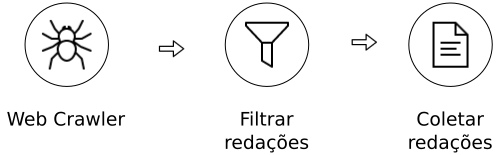
\includegraphics[scale=0.60]{images/metodologia_1.png}
\end{center}
\caption{O \textit{crawler}, navega entre as páginas HTML do banco de redações 
de forma metódica e automatizada indexando textos que posteriormente serão 
filtrados, coletados e armazenados.}
\label{figure:metodologia_1}
\end{figure}

\subsection{Balanceamento de dados}
\label{subsection:balanceamento_dados}

Em muitos domínios, os conjuntos de dados são naturalmente desbalanceados, 
dados desbalanceados representam o domínio onde qualquer classe de um grupo 
de dados, está representado por um amplo número de exemplos, enquanto as demais 
classes são representadas por poucos exemplos. Abordagens ao nível de dados 
equilibram a distribuição das classes no conjunto de dados, usar técnicas como 
\textit{undersampling} e \textit{oversampling}, resolvem o problema do 
desbalanceamento, de acordo com o estudo de \citeonline{ferreiraestudo}. A 
técnica \textit{oversampling} replica de forma aleatória, exemplos da classe 
minoritária, enquanto a técnica \textit{undersampling}, utilizada neste estudo, 
elimina aleatoriamente exemplos da classe majoritária. Além disso, 
\citeonline{machado2009estudo} em seu estudo, indica o uso das técnicas de 
limpeza de dados de modo a, eliminar os exemplos ruidosos e \textit{limítrofes}, 
respectivamente (\textit{class-label noise}, \textit{borderlines}). A figura 
\ref{figure:metodologia_2} ilustra a etapa onde os dados naturalmente 
desbalanceados são submetidos a técnica \textit{undersampling} e limpeza de 
dados, resultando um \textit{dataset} menor e balanceado.

\begin{figure}[H]
\begin{center}
    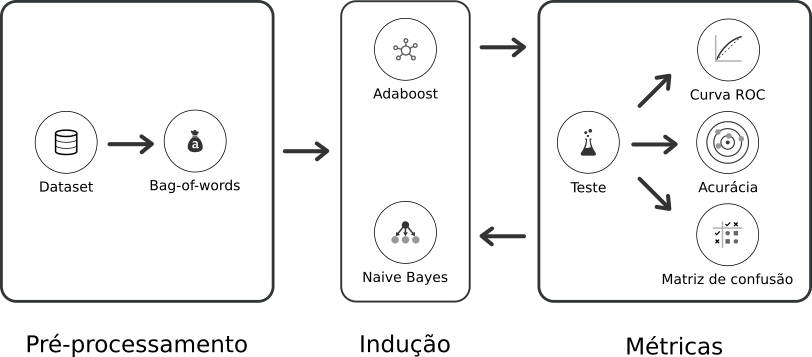
\includegraphics[scale=0.60]{images/metodologia_2.png}
\end{center}
\caption{O \textit{dataset} desbalanceado é submetido a técnica
\textit{undersampling} que gera um \textit{dataset} menor e balanceado.}
\label{figure:metodologia_2}
\end{figure}

% \newpage
\subsection{Pré-processamento, inferência indutiva e métricas de desempenho}
\label{subsection:pre_processamento}

A figura \ref{figure:metodologia_3}, ilustra as etapas necessárias para 
pré-processamento, indução e testes dos algoritmos classificadores. Devido à 
natureza textual não estruturada dos textos contidos no \textit{dataset}, no 
primeiro passo, os documentos armazenados necessitam de um pré-processamento. 
Cada sentença do texto é separada em \textit{tokens}, para transformar esses 
dados não estruturados em um formato estruturado, especificamente, uma tabela 
atributo-valor, denominada \textit{bag-of-words}. Nesta abordagem, palavras 
pouco significativas como artigos, preposições e conjunções, que pouco 
caracterizam o texto, podem ser ignoradas com uma ou mais listas de 
\textit{stopwords}. Segundo \citeonline{matsubara2003pretext}, este passo é 
importante, visto que a representação desses textos tem uma influência 
fundamental no resultado da indução dos algoritmos de Aprendizado de Máquina. 
No segundo passo, é necessário definir os parâmetros da inferência indutiva de 
cada algoritmo e induzir os modelos classificadores \textit{Adaboost} e 
\textit{Naive Bayes}. O terceiro e último passo, o resultado da inferência dos 
classificadores são avaliados com as principais métricas de análise de 
classificadores citadas na literatura de Aprendizado de Máquina. Os passos dois 
e três são repetidos até que um dos classificadores apresente resultados 
relevantes ao estudo.

\begin{figure}[H]
\begin{center}
    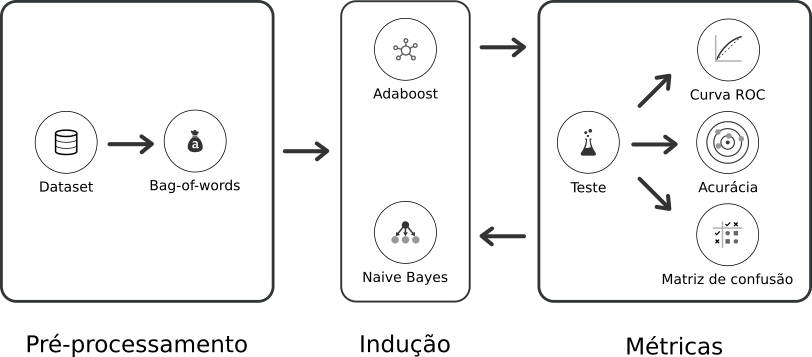
\includegraphics[scale=0.60]{images/metodologia_3.png}
\end{center}
\caption{O \textit{dataset} balanceado é submetido a técnica 
\textit{bag-of-words} no pré-processamento, resultando em uma estrutura de 
atributo-valor utilizada na inferência indutiva do classificadores, por fim, os 
modelos induzidos são avaliados por métricas de desempenho.}
\label{figure:metodologia_3}
\end{figure}

% \newpage
\subsection{Validação cruzada}
\label{subsection:validacao_cruzada}

Para avaliar e validar a hipótese proposta, foi adotada a metodologia de 
validação cruzada. O estudo de \citeonline{tavares2007estudo}, explica que esta 
abordagem consiste em fracionar o \textit{dataset} em \textbf{N} partes 
(\textit{folds}). Destas, \textbf{N}-1 partes são aplicadas na inferência 
indutiva e uma amostra é utilizada como base de testes. O método é repetido 
\textbf{N} vezes, de forma que cada fração seja utilizada apenas uma vez como 
conjunto de testes. Por fim, o resultado final é calculado pela média dos 
resultados atingidos em cada ciclo, obtendo-se assim uma estimativa da 
qualidade da inferência induzida, o que permite análises estatísticas. A Figura 
\ref{figure:metodologia_4} ilustra o fracionamento do \textit{dataset} em 
\textbf{N} partes, da qual, uma amostra é separada para testes e as demais para 
inferência indutiva, ao fim, é calculada a média dos resultados obtidos de cada 
métrica de desempenho. 

\begin{figure}[H]
\begin{center}
    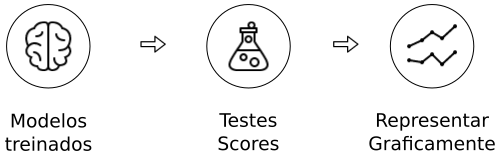
\includegraphics[scale=0.50]{images/metodologia_4.png}
\end{center}
\caption{O \textit{dataset} balanceado é fracionados en N partes, sendo uma 
parte separada para testes e as demais utilizada na indução dos classificadores, 
por fim, é calculada a média dos resultados obtidos.}
\label{figure:metodologia_4}
\end{figure}